\documentclass[a4paper, 10pt]{article}
\usepackage[a4paper,left=3cm,right=2cm,top=2.5cm,bottom=2.5cm]{geometry}
\usepackage[utf8]{inputenc} % Change according your file encoding
\usepackage{graphicx}
%\usepackage[demo]{graphicx}
\usepackage{url}

\usepackage{float}
\usepackage{amsmath}
\usepackage{xcolor}
\usepackage{todonotes}

\usepackage{listings}

\definecolor{backcolour}{rgb}{0.95,0.95,0.92}

\lstdefinestyle{mystyle}{
    backgroundcolor=\color{backcolour},  
    breakatwhitespace=false,         
    basicstyle=\scriptsize,
    breaklines=true,                 
    captionpos=b,                    
    keepspaces=true,                 
    showspaces=false,                
    showstringspaces=false,
    showtabs=false,                  
    tabsize=2,
    frame=single
}



\lstset{style=mystyle}

%opening
\title{Seminar Report: Opty}
\author{\textbf{Ignacio Encinas Rubio, Adrián Jimenez González}}
\date{\normalsize\today{}}

\begin{document}

\maketitle

%\begin{center}
  %Upload your report in PDF format.
  
  %Use this LaTeX template to format the report.
  
	%A compressed file (.tar.gz) containing all your source code files must be submitted together with this report.
%\end{center}

\section{Introduction}


\textit{Introduce in a couple of sentences the seminar and the main topic related to distributed systems it covers.}

\section{Code modifications}

   In this section we will briefly comment the code added to the template version in order to
   make the algorithm work. We will show the minimum number of lines of code possible to follow the reasoning.

  \subsection{Entry.erl}

    \begin{minipage}{.45\textwidth}
	\begin{lstlisting}[language=erlang, caption={Template}]
entry(Value, Time) ->
    receive
        {read, Ref, From} ->
            %% TODO: ADD SOME CODE
            entry(Value, Time);
        {write, New} ->
            entry(... , make_ref()); 
        {check, Ref, Readtime, From} ->
            if 
                 ... == ... ->  
                    %% TODO: ADD SOME CODE
                true ->
                    From ! {Ref, abort}
            end,
            entry(Value, Time);
        stop ->
            ok
    end.
 	\end{lstlisting}
    \end{minipage}\hfill
    \begin{minipage}{.45\textwidth}
	\begin{lstlisting}[language=erlang, caption={Filled version}]
entry(Value, Time) ->
    receive
        {read, Ref, From} ->
	    From ! {Ref, self(), Value, Time},
            entry(Value, Time);
        {write, New} ->
            entry(New , make_ref());
        {check, Ref, Readtime, From} ->
            if 
                 Readtime == Time -> 
		    From ! {Ref, ok};
                true ->
                    From ! {Ref, abort}
            end,
            entry(Value, Time);
        stop ->
            ok
    end.
  	\end{lstlisting}
  \end{minipage}

In this module we need to complete the \textbf{entry} function. This function is the responsible of the behaviour of the entries. The fuction will receive 3 types of message: read, write and check. 

\begin{itemize}
  \item  In case it receive a read message we will send a message with \textit{Value}, a timestamp and our PID.
  \item In case we receive a write message we will just update the \textit{Value}. 
  \item Finnaly, in case we receive a check message, we must compare \textit{Readtime} of the message with our timestamp, if it is the same, we send a ok message (commit), else we send an abort message.
\end{itemize}


\subsection{Handler.erl}

  \begin{minipage}{.45\textwidth}
	\begin{lstlisting}[language=erlang, caption={Template}]
handler(Client, Validator, Store, Reads, Writes) ->         
    receive
        {read, Ref, N} ->
            case lists:keyfind(..., ..., ...) of  %% TODO: COMPLETE
                {N, _, Value} ->
                    %% TODO: ADD SOME CODE
                    handler(Client, Validator, Store, Reads, Writes);
                false ->
                    %% TODO: ADD SOME CODE
                    %% TODO: ADD SOME CODE
                    handler(Client, Validator, Store, Reads, Writes)
            end;
        {Ref, Entry, Value, Time} ->
            %% TODO: ADD SOME CODE HERE AND COMPLETE NEXT LINE
            handler(Client, Validator, Store, [...|Reads], Writes);
        {write, N, Value} ->
            %% TODO: ADD SOME CODE HERE AND COMPLETE NEXT LINE
            Added = lists:keystore(N, 1, ..., {N, ..., ...}),
            handler(Client, Validator, Store, Reads, Added);
        {commit, Ref} ->
            %% TODO: ADD SOME CODE
        abort ->
            ok
    end.
 	\end{lstlisting}
    \end{minipage}\hfill
    \begin{minipage}{.45\textwidth}
	\begin{lstlisting}[language=erlang, caption={Filled version}]
handler(Client, Validator, Store, Reads, Writes) ->         
    receive
        {read, Ref, N} ->
            case lists:keyfind(N, 1, Writes) of  
                {N, _, Value} ->
		    Client ! {value, Ref, Value},
                    handler(Client, Validator, Store, Reads, Writes);
                false ->
		    Entry = store:lookup(N, Store),
		    Entry ! {read, Ref, self()},
                    handler(Client, Validator, Store, Reads, Writes)
            end;
        {Ref, Entry, Value, Time} ->
	    Client ! {value, Ref, Value},
            handler(Client, Validator, Store, [{Entry, Time}|Reads], Writes);
        {write, N, Value} ->
	    Entry = store:lookup(N, Store),
            NewWrites = lists:keystore(N, 1, Writes, {N, Entry, Value}),
            handler(Client, Validator, Store, Reads, NewWrites);
        {commit, Ref} ->
	    Validator ! {validate, Ref, Reads, Writes, Client};
        abort ->
            ok
    end.
  	\end{lstlisting}
  \end{minipage}

The next function we need to fil is on Handler module. The \textbf{handler} function expects to receive 4 types of messages: read, reply of entry, write and commit message.

\begin{itemize}
  \item If the message is read, we need to see if we have already written to this entry before using N, 1 and Writes as parameters for keyfind function. In case that is true, we will send \textit{Value} to the Client. Else, we look for the corresponding N Entry and we send a read message to the handler.
  \item In case we recieve a reply of an Entry, we need to seend teh reading value of the Entry to the Client. Also we need to add this Read to the Client's Reads.
  \item If the message is write, we look up for an entry and we need to append or update if existed the entry in our Writes list.
  \item Last message we can receive is commit. With that message we need to send a validate message to the Validator with with \textit{Ref, Reads, Writes and Client} values.
\end{itemize}

\clearpage
\subsection{Validator.erl}

In the validator module we have 3 functions to complete. 

\begin{minipage}{.45\textwidth}
	\begin{lstlisting}[language=erlang, caption={Template}]

validator() ->
    receive
        {validate, Ref, Reads, Writes, Client} ->
            Tag = make_ref(),
            send_read_checks(..., Tag),  %% TODO: COMPLETE
            case check_reads(..., Tag) of  %% TODO: COMPLETE
                ok ->
                    update(...),  %% TODO: COMPLETE
                    Client ! {Ref, ok};
                abort ->
                    %% TODO: ADD SOME CODE
            end,
            validator();
        stop ->
            ok;
        _Old ->
            validator()
    end.
 	\end{lstlisting}
    \end{minipage}\hfill
    \begin{minipage}{.45\textwidth}
	\begin{lstlisting}[language=erlang, caption={Filled version}]

validator() ->
    receive
        {validate, Ref, Reads, Writes, Client} ->
            Tag = make_ref(),
            send_read_checks(Reads, Tag),  
            case check_reads(length(Reads), Tag) of  
                ok ->
                    update(Writes),
                    Client ! {Ref, ok};
                abort ->
		    Client ! {Ref, abort}
            end,
            validator();
        stop ->
            ok;
        _Old ->
            validator()
    end.
  	\end{lstlisting}
  \end{minipage}


The \textbf{validator} function we wait for a validate message. When we receive that message we need to check the request to every entry we have read and check the results.

\begin{itemize}
  \item In case the case the transaction is OK, we flush writes and finish with a ok message to the Client.
  \item In case we read stale data, we send to the Client an abort message.
\end{itemize}

\begin{minipage}{.45\textwidth}
	\begin{lstlisting}[language=erlang, caption={Template}]

update(Writes) ->
    lists:foreach(fun({_, Entry, Value}) -> 
                  %% TODO: ADD SOME CODE
                  end, 
                  Writes).
 	\end{lstlisting}
    \end{minipage}\hfill
    \begin{minipage}{.45\textwidth}
	\begin{lstlisting}[language=erlang, caption={Filled version}]

update(Writes) ->
    lists:foreach(fun({_, Entry, Value}) -> 
		  Entry ! {write, Value}
                  end, 
                  Writes).
  	\end{lstlisting}
  \end{minipage}


  The next fuction to complete is \textbf{update}. In this fuction we need to send a write message to Entry with the corresponding Value.


\begin{minipage}{.45\textwidth}
	\begin{lstlisting}[language=erlang, caption={Template}]
send_read_checks(Reads, Tag) ->
    Self = self(),
    lists:foreach(fun({Entry, Time}) -> 
                  %% TODO: ADD SOME CODE
                  end, 
                  Reads).
 	\end{lstlisting}
    \end{minipage}\hfill
    \begin{minipage}{.45\textwidth}
	\begin{lstlisting}[language=erlang, caption={Filled version}]

send_read_checks(Reads, Tag) ->
    Self = self(),
    lists:foreach(fun({Entry, Time}) -> 
		  Entry ! {check, Tag, Time, Self}
                  end, 
                  Reads).
  	\end{lstlisting}
  \end{minipage}

Last function is \textbf{send\_read\_checks}. In this function we send to the Entry a check message with the Tag and Time for each existing Entry.

\clearpage

\subsection{Server.erl}

\begin{minipage}{.45\textwidth}
	\begin{lstlisting}[language=erlang, caption={Template}]
server(Validator, Store) ->
    receive 
        {open, Client} ->
            %% TODO: ADD SOME CODE
            server(Validator, Store);
        stop ->
            Validator ! stop,
            store:stop(Store)
    end.
 	\end{lstlisting}
    \end{minipage}\hfill
    \begin{minipage}{.45\textwidth}
	\begin{lstlisting}[language=erlang, caption={Filled version}]

server(Validator, Store) ->
    receive 
        {open, Client} ->
	    Client ! {transaction, Validator, Store},
            server(Validator, Store);
        stop ->
            Validator ! stop,
            store:stop(Store)
    end.
  	\end{lstlisting}
  \end{minipage}

  The last module we have to modify is \textbf{server}. In this case \textit{server} function is waiting for open message. When we receive that message, we send to the Client the Validator and Store for the transaction.

\clearpage
\section{Performance}

We have used a shell script to automatize the testing and make the results easily reproducible. Every plot shows error bars for every point, but they are so small that they are not noticeable in most cases.

As indicated by the assignment we've tried to pick free parameters for each test in a way that lets us see the effect of the parameter under study. 

\subsection{Number of concurrent clients in the system}
\label{sec:numclients}

Increasing the number of clients makes it easier for them to clash, so it decreases the mean success rate pretty fast.

\begin{figure}[H]
  \centering
  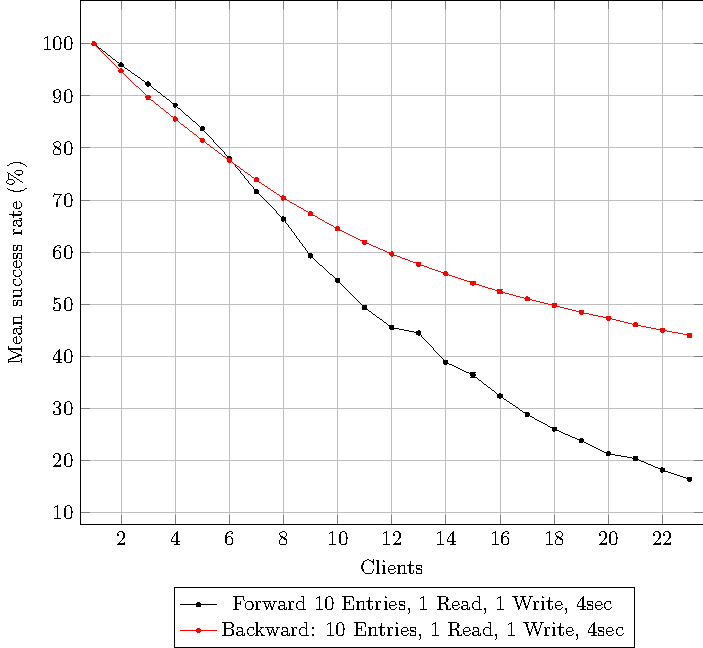
\includegraphics[width=0.95\linewidth]{plots/numclients.pdf}
    \caption{Success rate w.r.t nº of clients}
    \label{fig:numclients}
\end{figure} 



\clearpage
\subsection{Number of entries in the store}
\label{sec:numentries}
This is perhaps the most tricky parameter of our system. It shows extremely complex behaviour for some corner cases.

On the other hand, it is also true that our intuition holds for the majority of cases. That is, whenever $\text{entries} \gg \text{clients}$. Increasing the number of entries decreases the possibility of conflict, so it increases the success rate.
\begin{figure}[H]
  \centering
  \includegraphics[width=0.95\linewidth]{plots/numentries.pdf}
    \caption{Success rate w.r.t nº of entries}
    \label{fig:numentries}
\end{figure} 

\clearpage
\subsection{Number of reads per transaction}
\label{sec:numreads}
Doing more reads makes it easier for other clients to update those entries we've used and invalidate our transactions.

\begin{figure}[H]
  \centering
  \includegraphics[width=0.95\linewidth]{plots/numreads.pdf}
    \caption{Success rate w.r.t nº of reads}
    \label{fig:numreads}
\end{figure} 

\clearpage
\subsection{Number of writes per transaction}
\label{sec:numwrites}
Doing more writes increases the probability of updating an entry that had been previously read by other transaction that had not finished before we commited, so it decreases the success rate.

\begin{figure}[H]
  \centering
  \includegraphics[width=0.95\linewidth]{plots/numwrites.pdf}
    \caption{Success rate w.r.t nº of writes}
    \label{fig:numwrites}
\end{figure} 

\clearpage
\subsection{Ratio of read/writes}
\label{sec:ratioreadwrites}

The conflicts appear whenever we read outdated data, so having very one sided transactions will result in almost no conflicts. The success rate decreases rapidly whenever we have a balanced transaction that performs both operations.

\begin{figure}[H]
  \centering
  \includegraphics[width=0.95\linewidth]{plots/ratio.pdf}
    \caption{Success rate w.r.t ratio of reads/writes with fixed amount of total operations}
    \label{fig:ratio}
\end{figure} 

\subsection{Different percentage of accessed entries w.r.t the total number of entries}
\label{sec:nose}
A small percentage of accessed entries obviously increases our success rate, as the possibility for conflict is lower. It is also worth noting that this also introduces high variability on the success rate as some clients will access very crowded subsets while others will not.
\begin{figure}[H]
  \centering
  \includegraphics[width=0.95\linewidth]{plots/subset.pdf}
    \caption{Success rate w.r.t percentage of Entries accessible by each client}
    \label{fig:subset}
\end{figure} 


\subsection{What is the impact of each of these parameters on the success rate?}
Increasing the number of clients, reads and writes reduces the success rate, while increasing the number of entries increases it.

The results are very intuitive, because more complex transactions have higher probability of conflicting with others by reading entries that have been written.


On the other hand, there are some special cases where this intuition falls apart such as the one examined at Section \ref{sec:magia}. Results at Section \ref{sec:numentries} also indicate that adding entries can decrease the success rate for a low count of clients that perform complex transactions.


\subsection{Is the success rate the same for the different clients?}
In every plot we show the standard deviation via error bars. They're so small it's difficult to see them, so mainly yes. The only where the clients get different success rates is in the one where they get a subset of accessed entries. It's expected as some clients will get subsets with very little \textit{traffic}, and other clients will compete with many others to access the same entries.

\clearpage
\subsection{Bonus. Minimum success rate per number of entries}
\label{sec:magia}
At first we can think that as we increase the number of clients the success rate will go to $0$. It's not such a wild idea but if we think carefully we'll notice that there is a pattern in our transactions that always succeeds: $\text{Write} \rightarrow \text{Read}$. This gives us a lower bound on the amount of transactions that will succeed, as shown in Figure \ref{fig:magia}. In the simple case we've studied, in the $50\%$ of cases our transaction will be a write followed by a read. In order for it to succeed, the read will have to access the entry we've previously written, so the probability of doing so is $\frac{1}{n}$, where $n$ is the number of entries.

Obviously as the transaction complexity increases the calculation required to obtain this lower bound does too so we can't go much further, but surely anyone skilled enough in combinatorics could.
\begin{figure}[H]
  \centering
  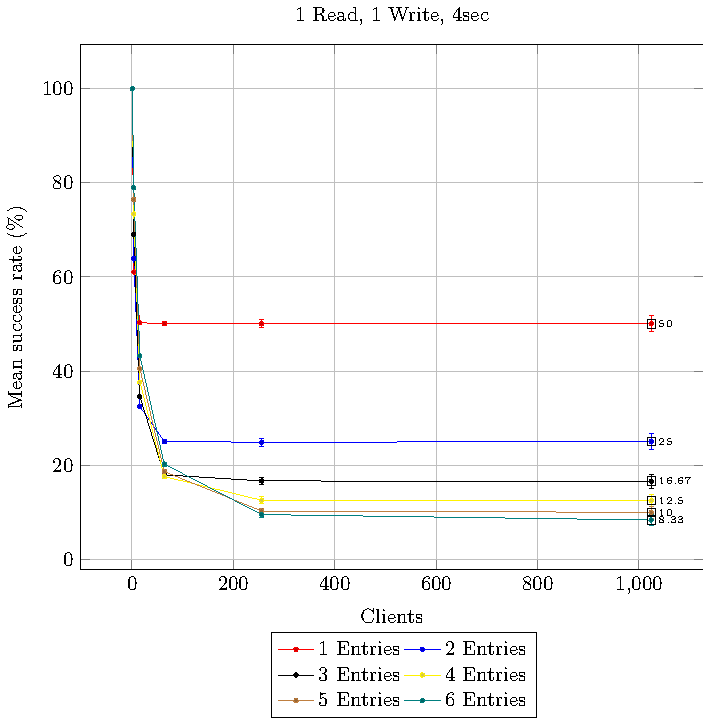
\includegraphics[width=0.95\linewidth]{plots/numentriesv2.pdf}
    \caption{Success rate w.r.t nº of clients and entries}
    \label{fig:magia}
\end{figure} 

This also helps explain the situation where adding entries does decrease the mean success rate. It's very unintuitive but considering this lower bound makes it much more obvious. When $\text{clients} \gg \text{entries}$ the conflicts will be unavoidable so the success rate will be very close to the lower bound, and increasing the number of entries decreases that lower bound significantly.

Obviously this is sort of a pathological example and it is not too representative. Surely the lower bound for any realistic transaction is so small that relying on this effect in order to sustain an acceptable lower bound makes no sense. Applying an algorithm for optimistic concurrency when you're expecting massive entry overload and contention would be pretty \textbf{bold}!

\clearpage

In order to check that our intuition is correct we've also checked with 2 Reads and 1 Write, where the expected lower bound would be $\displaystyle \frac{0.5}{n^2}$. The chance of starting the transaction with a write is still $50\%$ but now we have to hit the two consecutive reads in the same entry we read, thus getting a probability of $0.5 \cdot \frac{1}{n} \cdot \frac{1}{n}$. Figure \ref{fig:magia2} illustrates the expected trend. Similarly, we have replicated the results for other simple configurations.
\begin{figure}[H]
  \centering
  \includegraphics[width=0.95\linewidth]{plots/numclients2.pdf}
    \caption{Success rate w.r.t nº of clients and entries}
    \label{fig:magia2}
\end{figure} 

Overall, noticing this effect after discussing it in the labs session has been very enjoyable. Of course it is not of any practical use as we've already mentioned, but it shows how complex distributed systems are.


\clearpage
\section{Distributed execution}

For this experiment, we have made a few changes to generate a process in another node from one unique start function. The changes have been done in the \textit{opty} module. 

To be able to call the distributed server we have to register it and have it on the client side. We have used the piece of code from listing \ref{list:register}


\begin{minipage}{\textwidth}
  \begin{lstlisting}[language=erlang, caption={Register Distributed Server}, label={list:register}]
    spawn(Snode, fun() -> 
                         register(s, server:start(Entries))end),
  
 	\end{lstlisting}
\end{minipage}

Figures \ref{fig:2nodes}-\ref{fig:1node} it is shown the execution of the distributed algorithm. In the first one, we can see two nodes, in which we run clientside and serverside. In the right terminal, it is shown that \texttt{s} is created in the server node and the start function is executed in the client node (left terminal). 

Also, to show the correct behaviour, in figure \ref{fig:1node}, the server node is down and we can not spawn the server in that node, so the algorithm does not work.



\begin{figure}[H]
  \centering
  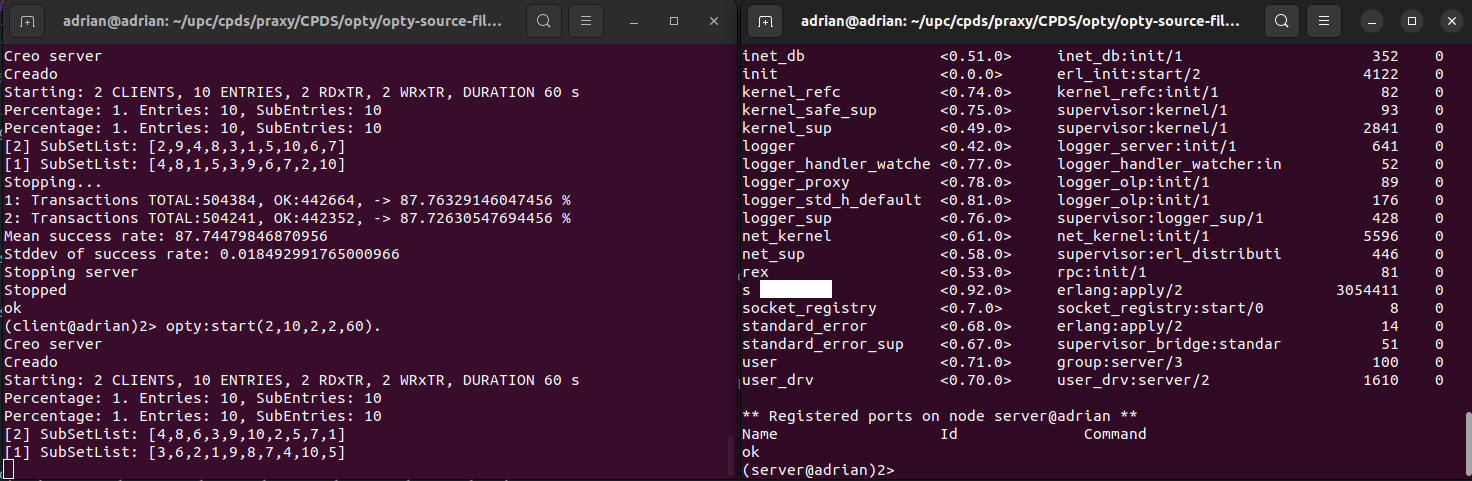
\includegraphics[width=0.95\linewidth]{images/optyWorking.png}
    \caption{Opty working in 2 nodes}
    \label{fig:2nodes}
\end{figure} 


\begin{figure}[H]
  \centering
  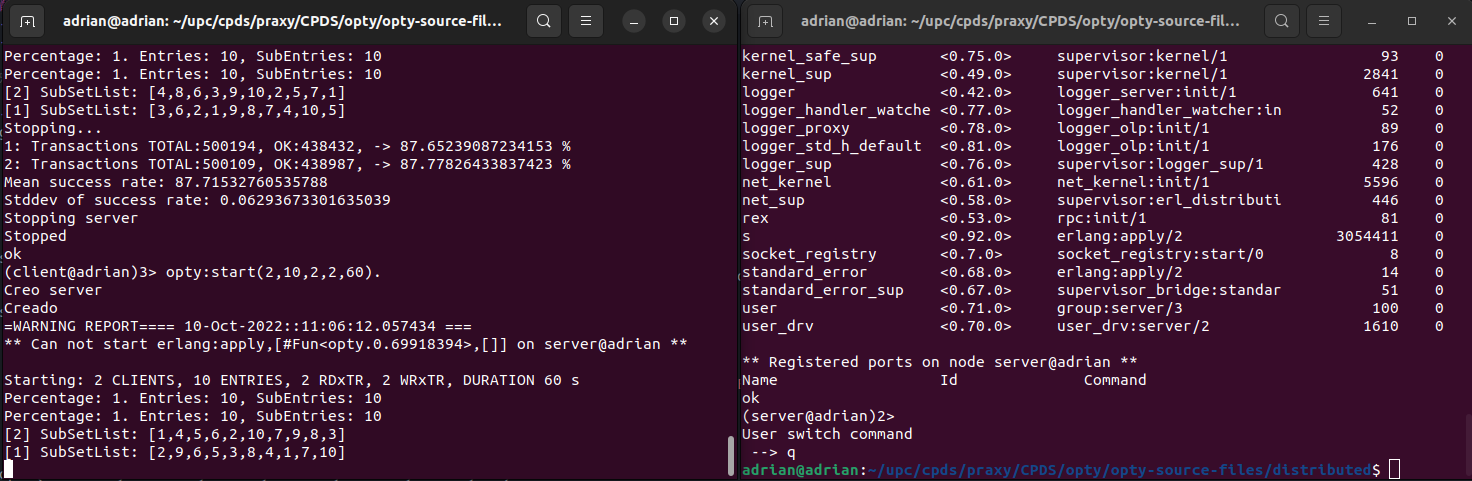
\includegraphics[width=0.95\linewidth]{images/opty1node.png}
    \caption{Opty failing with 1 node}
    \label{fig:1node}
\end{figure} 

\clearpage
\section{Other concurrency control techniques}


\subsection{Number of concurrent clients in the system}\label{timey-current-clients}

As we mentioned in Section \ref{sec:numclients}, in optimistic control, increasing the number of clients makes clashes more frequent, reducing the success ratio. When we increase the number of clients with timestamp control (timey), the number of clients also reduces the success ratio, but not that drastically, as it is shown in figure \ref{timey:numclients}. 

In the \textit{timey} algorithm, the writes tentatives are allocated in an ordered queue by the timestamp, being only discarded the transactions with older timestamps than the current version of the object (last read or written object).

\begin{figure}[H]
  \centering
  \includegraphics[width=0.95\linewidth]{timey_plots/numclients2.pdf}
    \caption{Success rate w.r.t nº of clients}
    \label{timey:numclients}
\end{figure} 

\clearpage
\subsection{Number of entries in the store}

The results show us that the bigger the number of entries for the number of clients, the best the success rate we obtain for both algorithms. \textit{Timey} algorithm results are better than \textit{opty} in the same conditions (same number of reads and writes per transaction). Even in corner cases as $\text{clients} \gg \text{entries}$, the success ratio is better. 

This behaviour is produced by the same cause explained in Section \ref{timey-current-clients}. The lower entries we have the more clashes we obtain. Results show that \textit{timey} has better tolerance.

\begin{figure}[H]
  \centering
  \includegraphics[width=0.95\linewidth]{timey_plots/numentries.pdf}
    \caption{Success rate w.r.t nº of entries}
    \label{timey:numentries}
\end{figure} 


\clearpage
\subsection{Number of reads per transaction}

Doing more reads per transaction decreases the success rate in the \textit{opty} algorithm. Differing from \textit{timey} algorithm behaviour, which maintains a ~98\% of success rate.

This difference is due to how \textit{timey} controls the read transactions. It will read the higher timestamp transaction that is lower than its timestamp, if the transaction is a tentative it will wait until that tentative is published. That mechanism allows the algorithm to not discard a large number of read transactions, only ones that have a lower timestamp than the last write transaction timestamp.

\begin{figure}[H]
  \centering
  \includegraphics[width=0.95\linewidth]{timey_plots/numreads.pdf}
    \caption{Success rate w.r.t nº of reads}
    \label{timey:numreads}
\end{figure} 

\clearpage
\subsection{Number of writes per transaction}

Doing more writes per transaction decreases the success rate in both algorithms. In both cases, we increase the probability of clashes. As the data shows, the \textit{timey} algorithm performs better in success rate for all the number of writes per transaction we have tested.

\begin{figure}[H]
  \centering
  \includegraphics[width=0.95\linewidth]{timey_plots/numwrites.pdf}
    \caption{Success rate w.r.t nº of writes}
    \label{timey:numwrites}
\end{figure} 

\clearpage
\subsection{Ratio of read/writes}

Studying the success rate taking into account the ratio of read/writes per instruction, we can say that both algorithms perform better with rates closer to the edges (0-100\%). In only-write (0\% of read operations) \textit{opty} performs better. Both algorithms decrease their success ratios with 10-30\% of read operations, although \textit{timey} performs better (around ~15\% as the maximum difference). From that point, increasing the ratio will produce an increased success ratio in \textit{timey} and maintaining the rate in \textit{opty}. Only in full-read transactions (100\% of reads operations), both algorithms match again.

\begin{figure}[H]
  \centering
  \includegraphics[width=0.95\linewidth]{timey_plots/ratio.pdf}
    \caption{Success rate w.r.t ratio of reads/writes with fixed amount of total operations}
    \label{timey:ratio}
\end{figure} 

\clearpage
\subsection{Different percentage of accessed entries w.r.t the total number of entries}

Both algorithms have the same behaviour. The lower the number of entries accessed, the higher the success rate. Fewer entries accessed per client implies having less probability of clashes between transactions. This impact is lower in \textit{timey}, in which we obtain smoother curvesin contrast \textit{opty}.

It is important to remark that \textit{timey} algorithm obtains better results in all the experiments we have done in this section, according to all the results of the experiments we have done previously.

\begin{figure}[H]
  \centering
  \includegraphics[width=0.95\linewidth]{timey_plots/subset.pdf}
    \caption{Success rate w.r.t percentage of Entries accessible by each client}
    \label{timey:subset}
\end{figure} 

\clearpage


\section{Forward validation}

To implement \textbf{forward validation} we need to modify the source code of some modules. These modules are handler, validator and entry. Validator and entry have the most changes to modify the behaviour of the checking phase. Meanwhile, handler only needs minor changes to match the structure of new messages to send to the validator and entries.

\subsection{Entry}

In this module, we have introduced a series of changes to accomplish forward validation. First of all, now we do not need to check when \textit{read} messages arrive. The validator will need to compare its Write list with the Reading list of the Entry. For that, we are going to implement a Reading list in Entry module, in which we will add the PID of the Handler every time it read (this implementation will need to take care of deleting all the appearances of that handler, discussed below).

With this change in \textit{read} messages, the behaviour on \textit{write} messages changes. Now, this kind of messages do not need to validate anything, so they will update directly.

\textit{Check} messages have the bigger change. They will change not only the structure but also all their behaviour. Now we check if the list of Reads is empty, which means that no one had read that entry so we are able to commit our transaction. Otherwise, we abort the transaction if there are some PID in our Read list. We are checking if there is an empty list because before checking validator asks for the entry for deleting the PID of the handler of the transaction.

The last type of message is \textit{delete}. This message deletes ALL the appearances of the requested PID from the Read list from the entry.

\subsection{Validator}

The validator module has a few changes in addition to the new entry messages structure. We are introducing some functions like "send\_write\_check" and "check\_writes", are responsible for sending check messages to the corresponding entries and receiving their answers to complete or abort the transactions.

Inside of \texttt{validator} function, we are waiting for a \textit{validate} message from the handler. The first we do (and the first change we find) is that validator asks for deleting ALL the appearances of the handler's PID from ALL the entries he is attempting to write. Then, it sends the checks messages with the previous functions, and depending on the response (ok or abort), it will update the Writes and accomplish successfully the transaction. Or it will abort the transaction. After these actions, the validator will need to delete also the Reads of that transaction in the corresponding entries in which the handler has read.

\subsection{Handler}

As mentioned before, this module only had some minor changes. They are focused on following the structure of the changed messages.

\subsection{Message Diagram}

To clarify the messages introduces, a diagram has been created. In figure \ref{fig:diagram} we can see the messages we are passing between the three modules we made changes and their structures.

\begin{figure}[H]
  \centering
  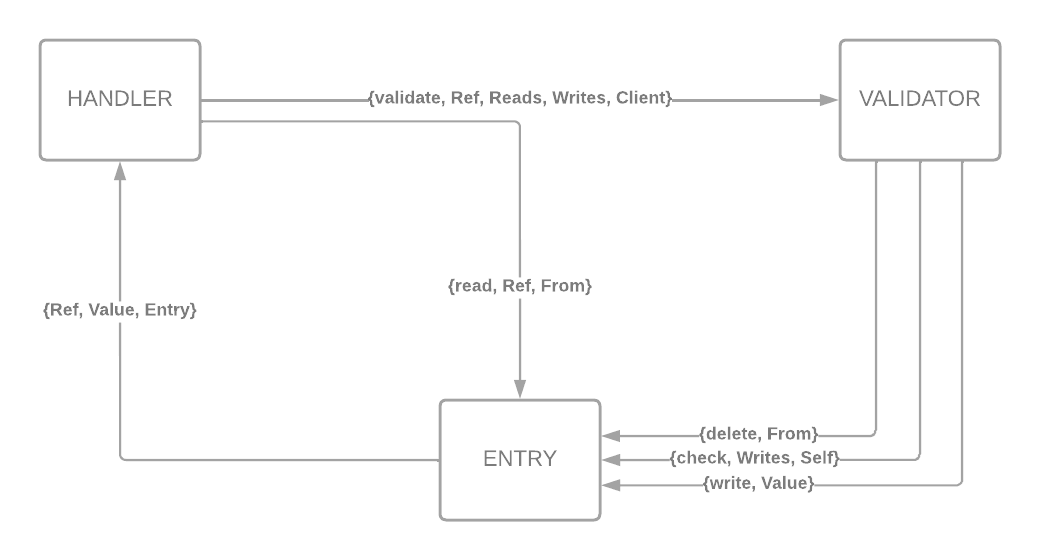
\includegraphics[width=0.95\linewidth]{images/messagesForward.png}
    \caption{Message diagram of Opty with Forward Validation}
    \label{fig:diagram}
\end{figure} 


\clearpage
\section{Personal opinion}

\subsection{Ignacio}

\subsection{Adrián}

In my opinion this practice have been interesting. I learned a bit more of Erlang and taking some challenges that previous practice didn't have. We have understand the opty algorithm and also timey to compare them. Also the main challenge (from my point of view) of modify the opty code without a "guide" code to implement forward validation, truly facing with Erlang language.

\end{document}
